\clearpage
%%=========================================
\section[Surface Analysis of Substrate C with Surface Pre-Growth Preparation]{Surface Analysis of Substrate C with Surface Pre-Growth Preparation%
    \sectionmark{Surface Analysis of Pre-Growth Substrate C}}\sectionmark{Surface Analysis of Pre-Growth Substrate C}\label{sec:subCb}

The ultimate goal for the \ac{mbe} preparation etch is to provide a clean, smooth, and well-ordered surface to minimise growth defects. As can be seen in Fig.~\ref{fig:subCb_om_df}, there are many features larger than \SI{0.5}{\micro\metre} on the surface. The density of those features is \SI{\sim 8e3}{\centi\metre^{-1}}. 

\begin{figure}[htbp]
    \centering
    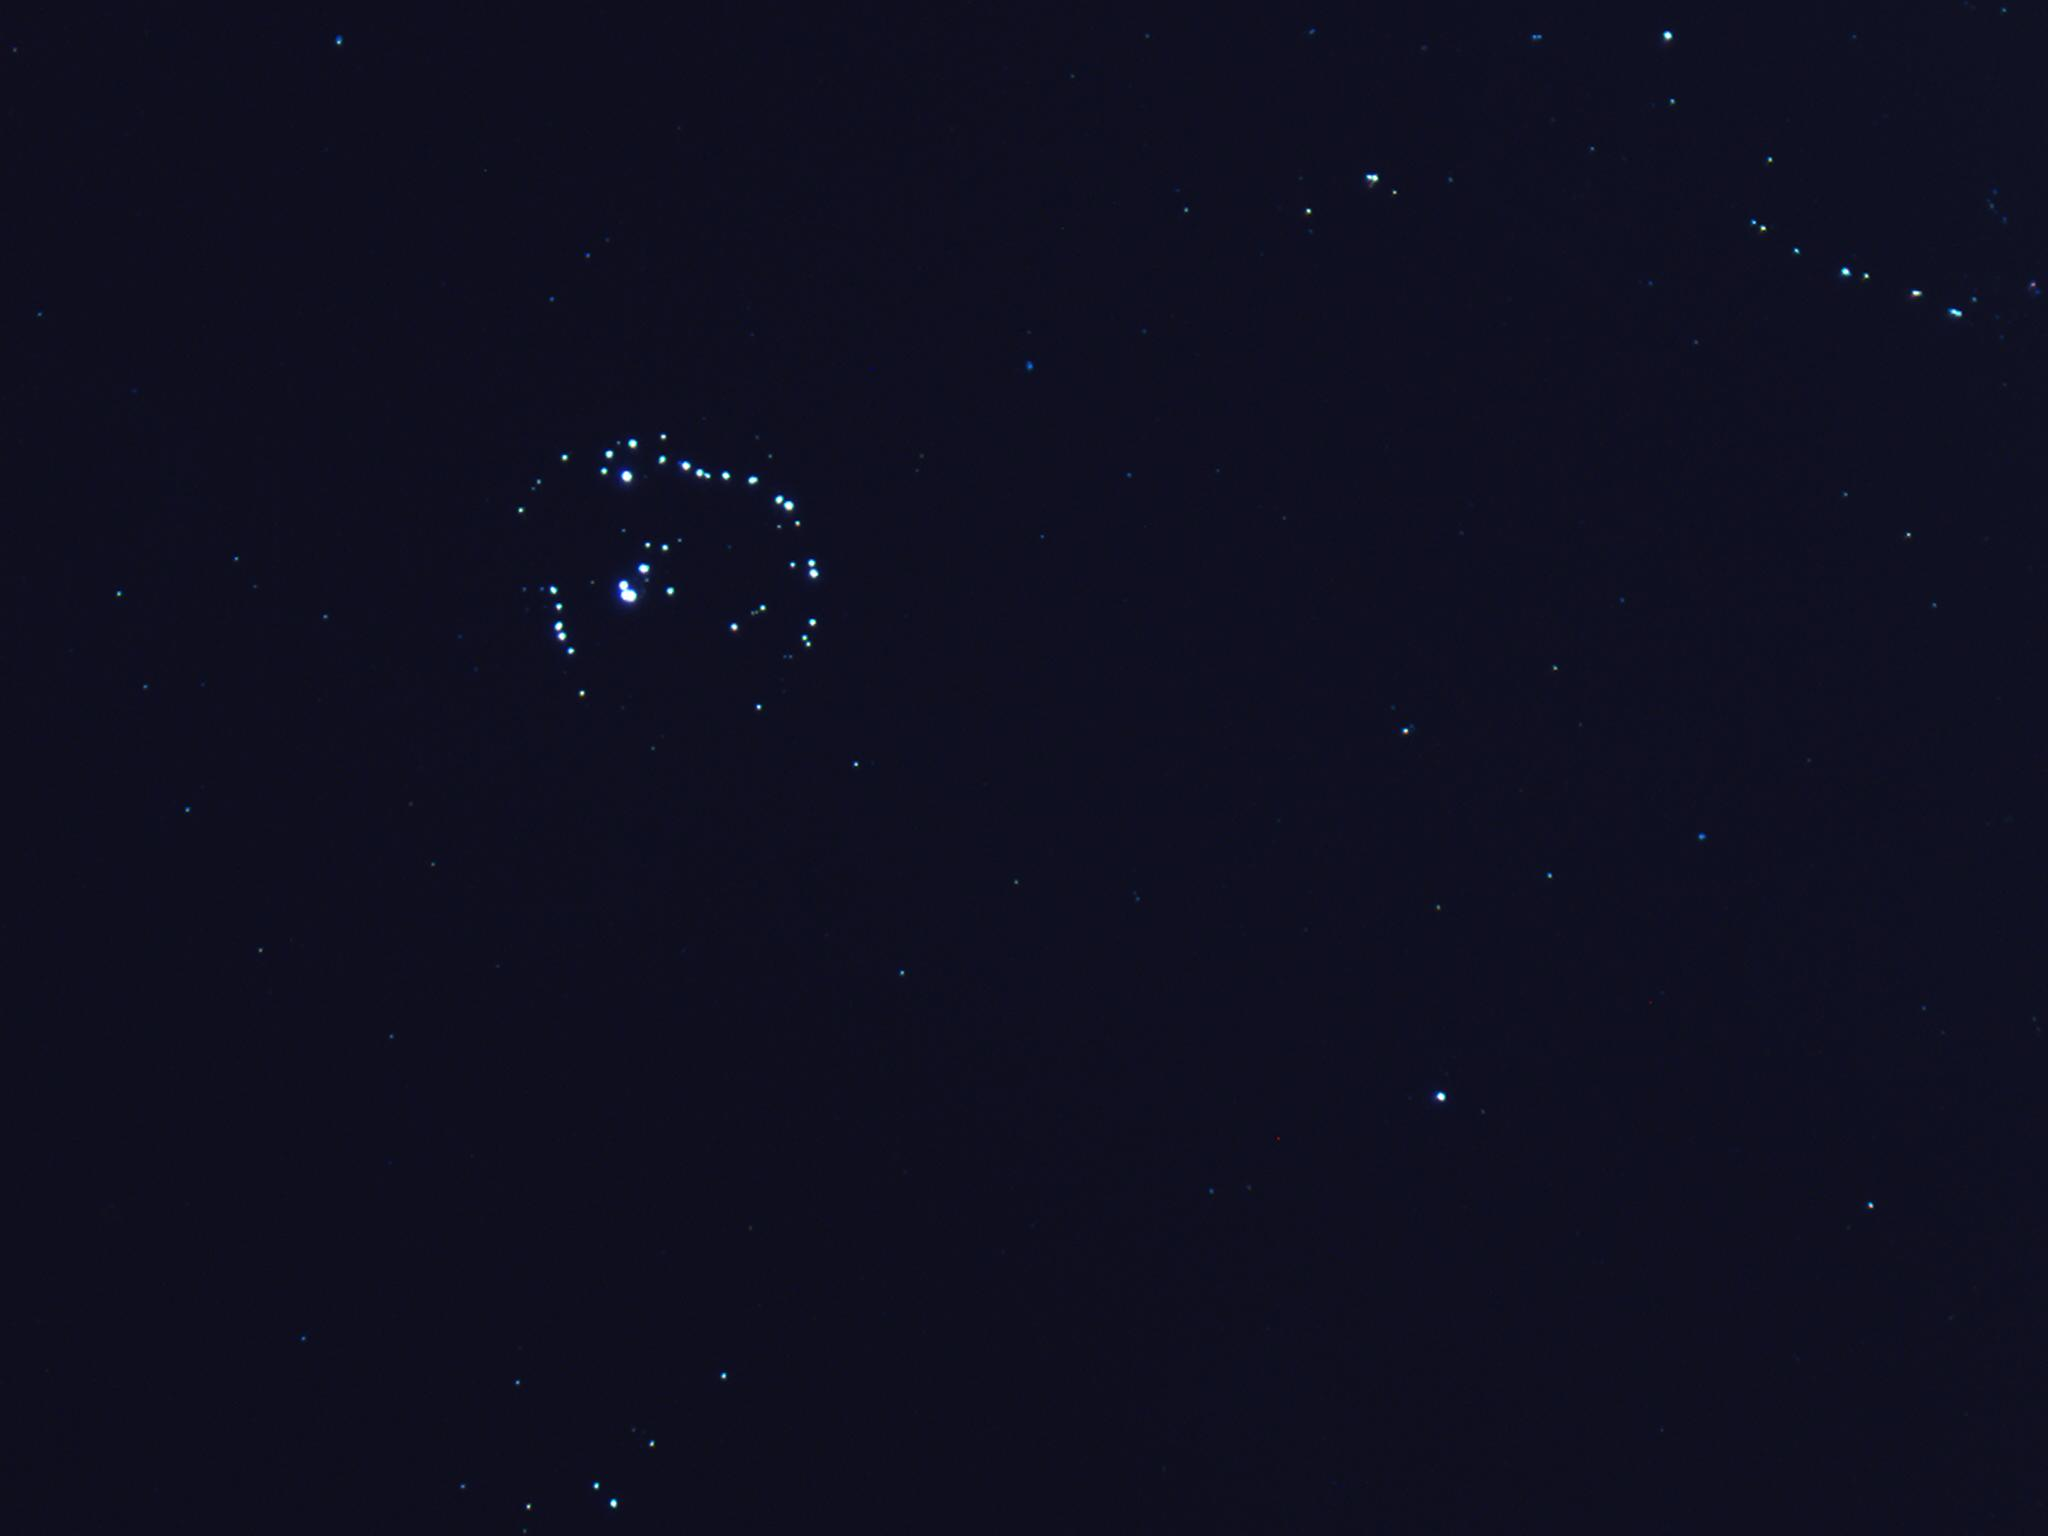
\includegraphics[width=0.8\linewidth]{subCb_om_df_n018_5x.jpg}
    \caption[Dark field optical microscopy image of substrate C with surface pre-growth preparation.]{Dark field optical microscopy image of substrate C with surface pre-growth preparation taken near the centre of the substrate.}\label{fig:subCb_om_df}
\end{figure}

\Ac{sem} shows the surface at a higher magnification and it reveals that there are much smaller particles distributed over the surface as well. Fig.~\ref{fig:subCb_sem_typical_centre} shows a typical image of an area near the centre of the substrate. Here the particle density is  \SI{1e+07}{\particle\centi\metre^{-2}}. The highest observed density of particles is counted near the upper right corner to be \SI{3e+07}{\particle\centi\metre^{-2}}, see Fig.~\ref{fig:subCb_sem_typical_corner}.

\begin{figure}[htbp]
    \begin{subfigure}[t]{0.49\textwidth}
        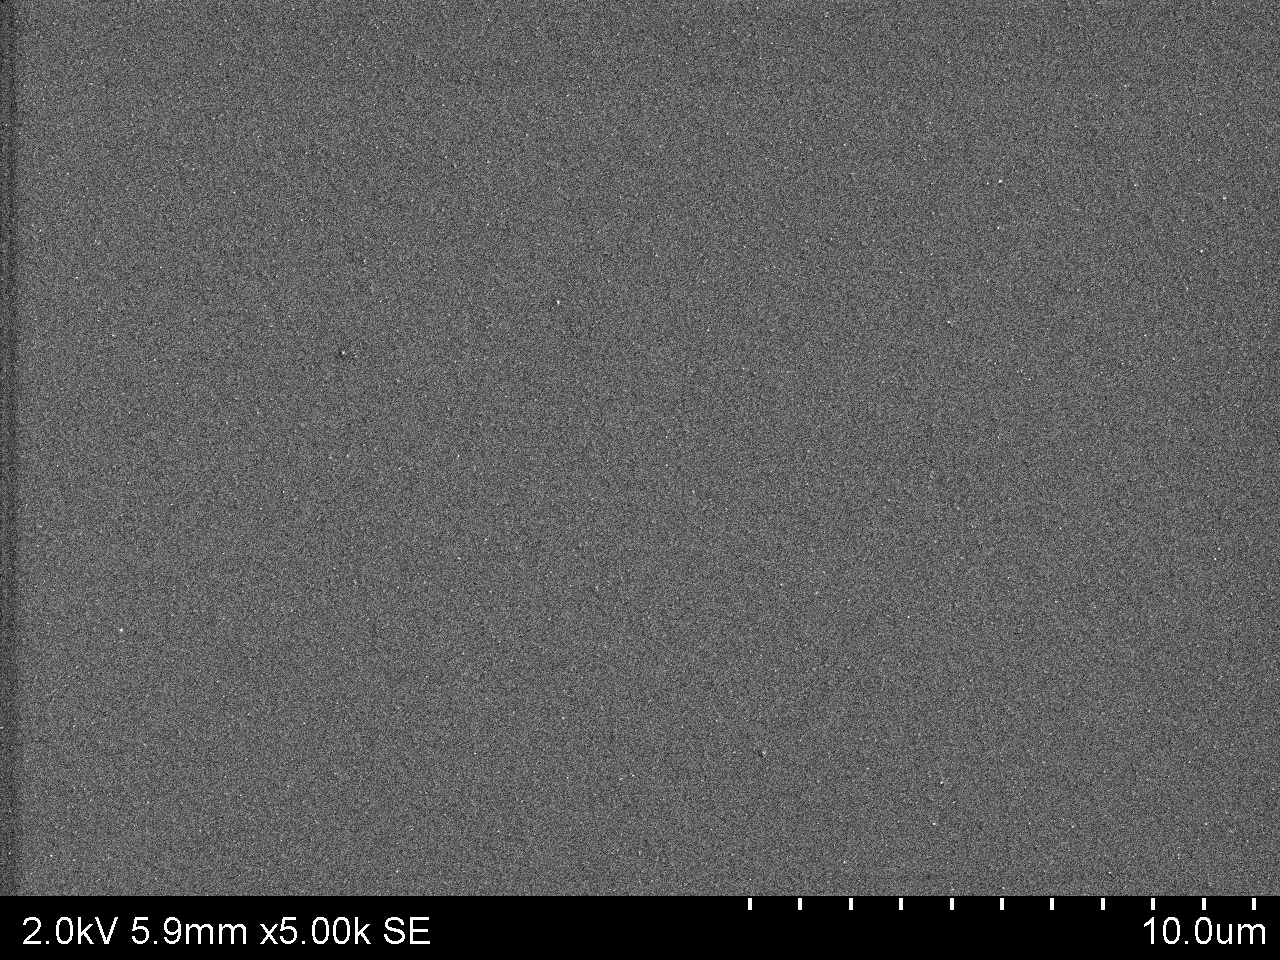
\includegraphics[width=\linewidth]{subCb_sem_04a_m008.png}
        \caption{}\label{fig:subCb_sem_typical_centre}
    \end{subfigure}%
    \hfill
    \begin{subfigure}[t]{0.49\textwidth}
        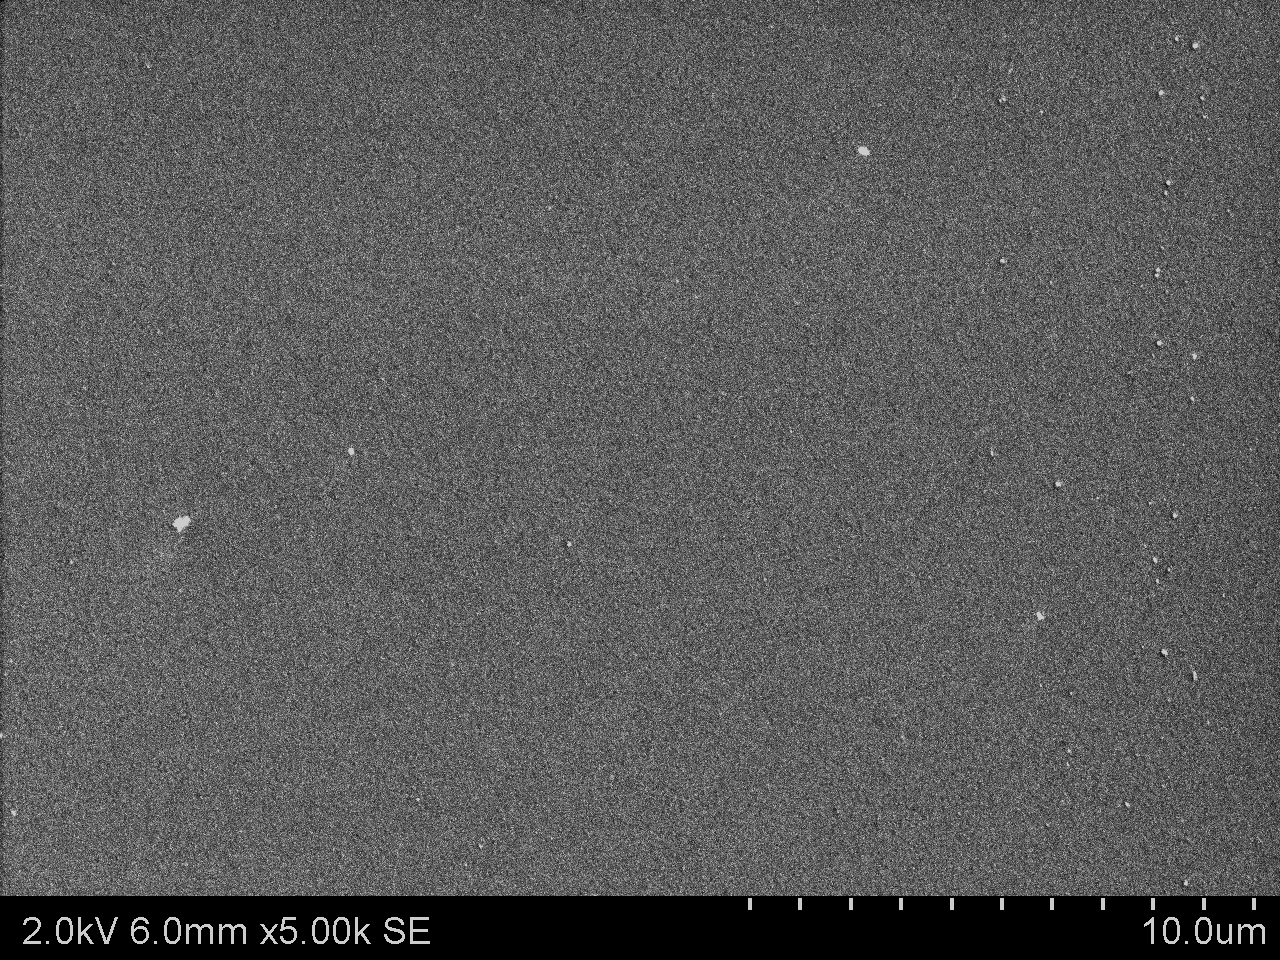
\includegraphics[width=\linewidth]{subCb_sem_04a_m005.png}
        \caption{}\label{fig:subCb_sem_typical_corner}
    \end{subfigure}%
    \caption[\Ac{sem} images of typical areas on substrate C with surface pre-growth preparation.]{\Acf{sem} images of \subref{fig:subCb_sem_typical_centre} a typical area near the centre and \subref{fig:subCb_sem_typical_corner} an area with a high density of particles near the edge of substrate C after surface pre-growth preparation.}\label{fig:subCb_sem_typical}
\end{figure}

%%=========================================
\subsection{Particles}

\begin{figure}
    \centering
    \begin{subfigure}[t]{\textwidth}
          \begin{minipage}[t]{0.43\linewidth}
            \centering
            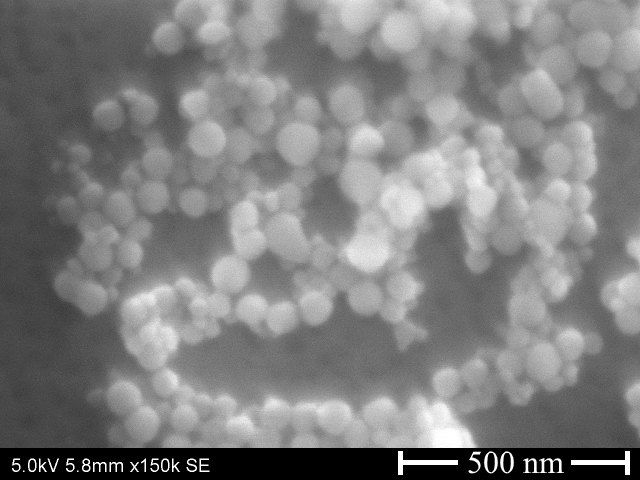
\includegraphics[width=\linewidth]{subCb_sem_07_m002.png}
          \end{minipage}
          \hfill
          \begin{minipage}[t]{0.43\linewidth}
            \centering
            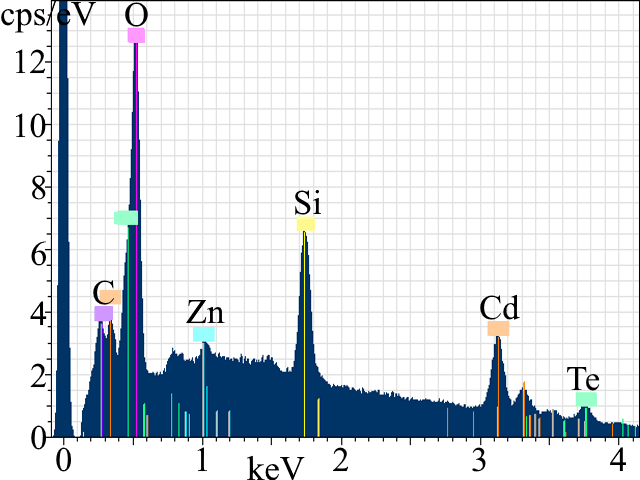
\includegraphics[width=\linewidth]{subCb_sem_07_m002_eds.png}
          \end{minipage}
          \begin{minipage}[t]{0.11\linewidth}
            \centering
            \atomicTable[&][&][&]
          \end{minipage}
        \caption{}\label{fig:subCb_silica}
    \end{subfigure}
    \par\bigskip
    \begin{subfigure}[t]{\textwidth}
          \begin{minipage}[t]{0.43\linewidth}
            \centering
            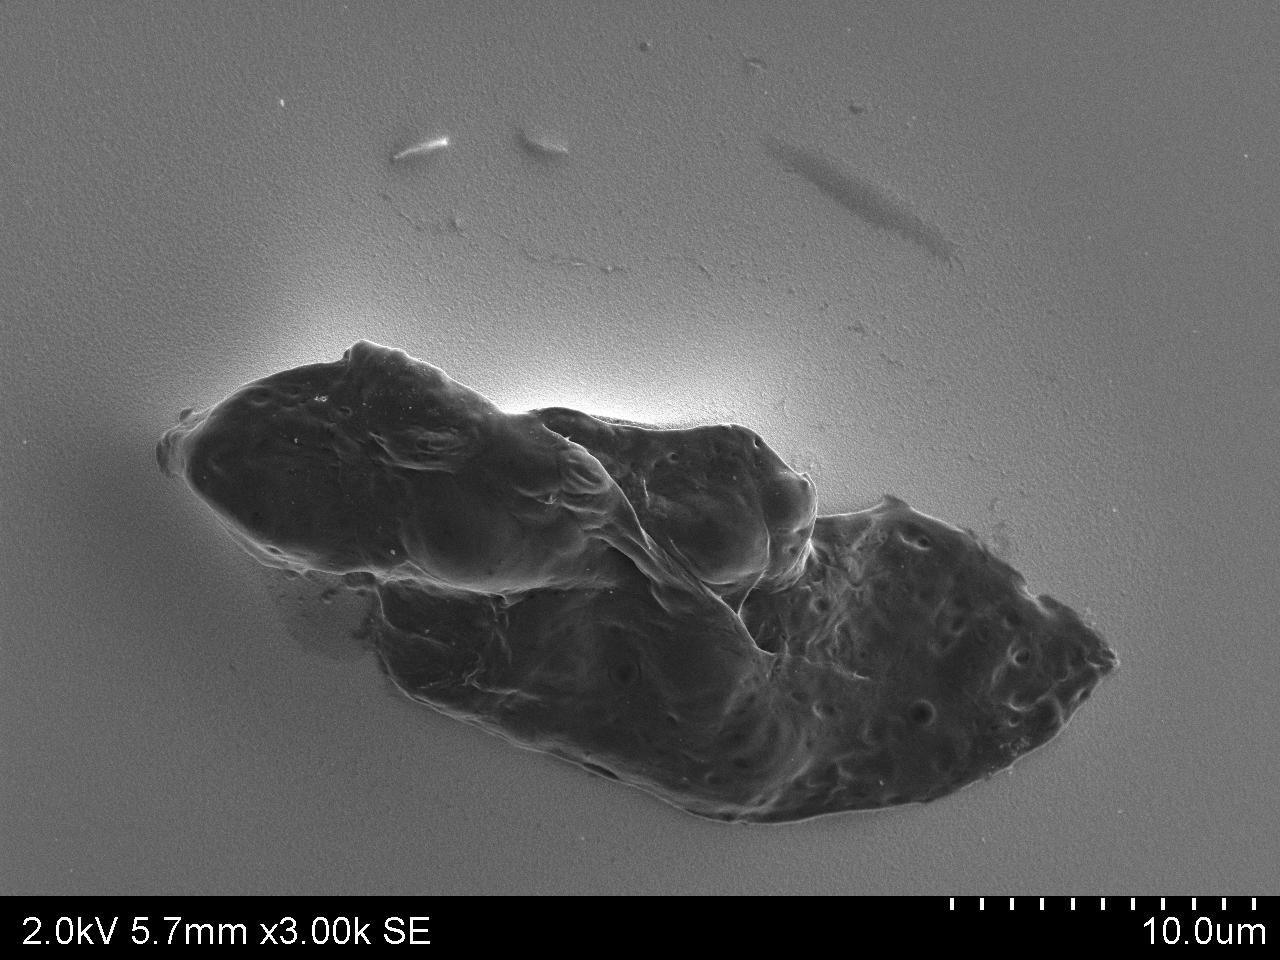
\includegraphics[width=\linewidth]{subCb_sem_03_m001.png}
          \end{minipage}
          \hfill
          \begin{minipage}[t]{0.43\linewidth}
            \centering
            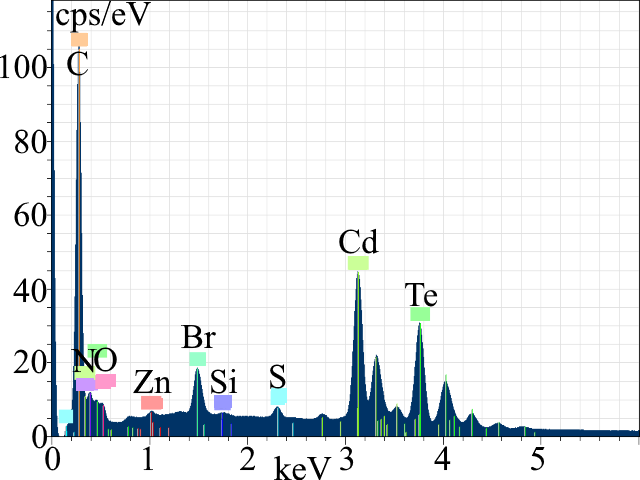
\includegraphics[width=\linewidth]{subCb_sem_03_m001_eds.png}
          \end{minipage}
          \begin{minipage}[t]{0.11\linewidth}
            \centering
            \atomicTable[&][&][&]
          \end{minipage}
        \caption{}\label{fig:subCb_Br-etch}
    \end{subfigure}
    \par\bigskip
    \begin{subfigure}[t]{\textwidth}
          \begin{minipage}[t]{0.43\linewidth}
            \centering
            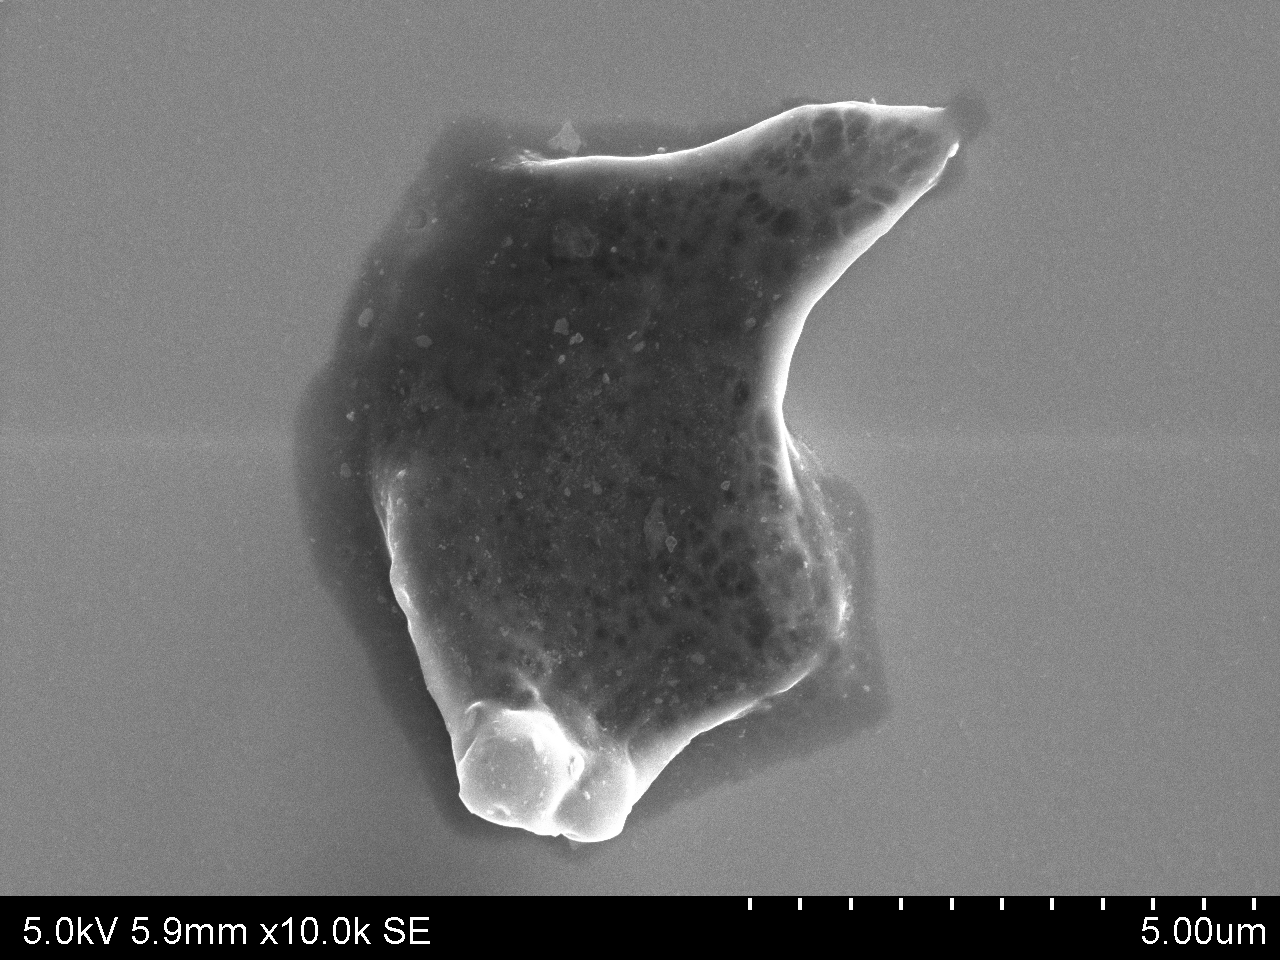
\includegraphics[width=\linewidth]{subCb_sem_09_m004.png}
          \end{minipage}
          \hfill
          \begin{minipage}[t]{0.43\linewidth}
            \centering
            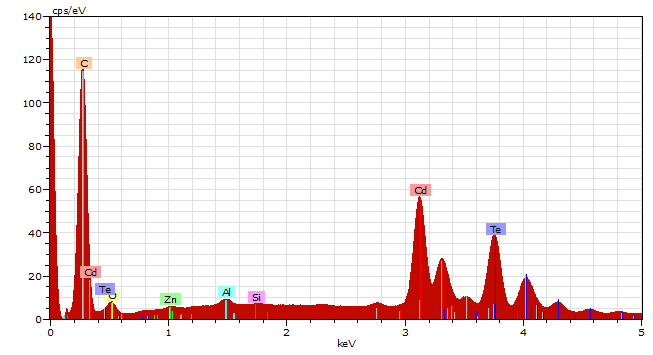
\includegraphics[width=\linewidth]{subCb_sem_09_m004_eds.png}
          \end{minipage}
          \begin{minipage}[t]{0.11\linewidth}
            \centering
            \atomicTable[&][&][&]
          \end{minipage}
        \caption{}\label{fig:subCb_Br-etch2}
    \end{subfigure}
    \caption[\Ac{sem} images, \ac{eds} spectra, and \ac{eds} atomic compositions of four different types of particles found on substrate C after surface pre-growth preparation.]{High resolution \acf{sem} images of four different types of particles found on substrate C after surface pre-growth preparation and the corresponding \acf{eds} spectra and atomic compositions: \subref{fig:subCb_silica} Silica (\ce{SiO2}) polishing grit; \subref{fig:subCb_Br-etch} particle with carbon, bromine, nitrogen, and sulphur; \subref{fig:subCb_Br-etch2} particle with carbon, bromine, and oxygen; and \subref{fig:subCb_silica_large} large silica agglomeration.}\label{fig:subCb_sem_w_eds}
\end{figure}
%
\begin{figure}[htbp]
\ContinuedFloat
    \centering
    \begin{subfigure}[t]{\textwidth}
          \begin{minipage}[t]{0.43\linewidth}
            \centering
            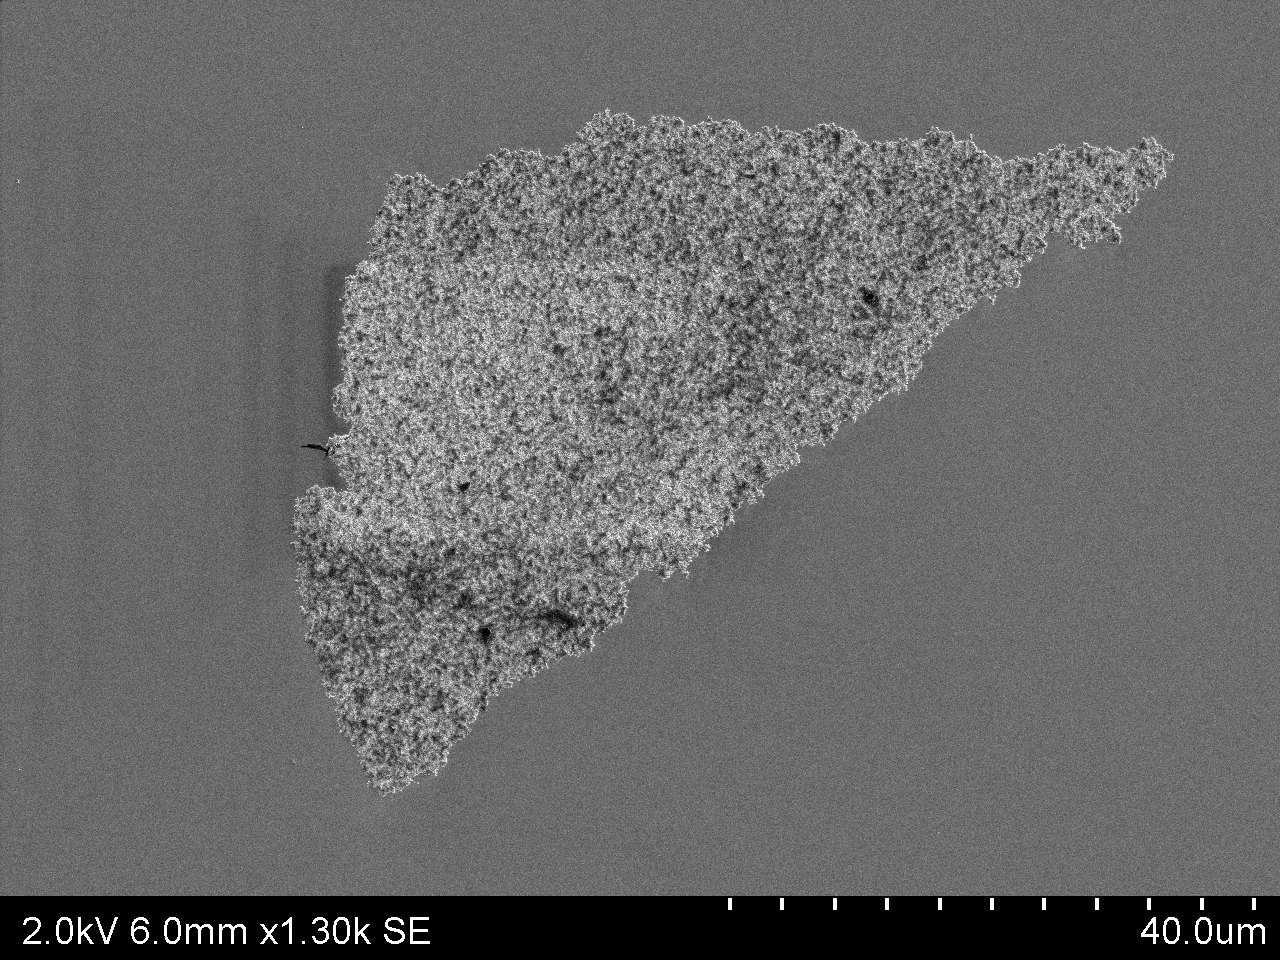
\includegraphics[width=\linewidth]{subCb_sem_03_m010.png}
          \end{minipage}
          \hfill
          \begin{minipage}[t]{0.43\linewidth}
            \centering
            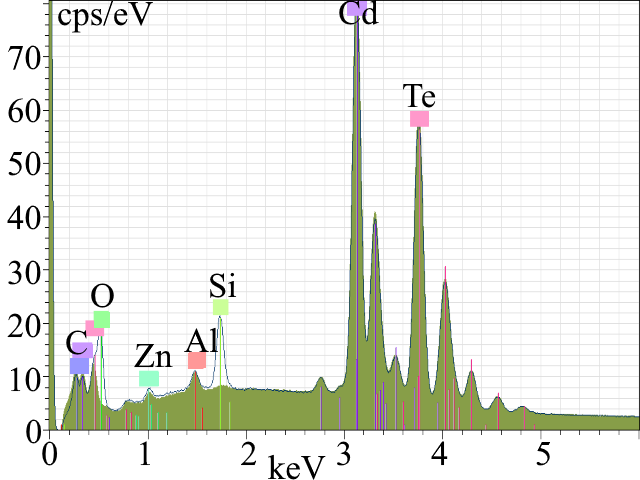
\includegraphics[width=\linewidth]{subCb_sem_03_m010_eds.png}
          \end{minipage}
          \begin{minipage}[t]{0.11\linewidth}
            \centering
            \atomicTable[&][&][&]
          \end{minipage}
        \caption{}\label{fig:subCb_silica_large}
    \end{subfigure}
    \captionsetup{list=no}
    \caption{\emph{(continued)}}
\end{figure}

\todo{The alumina polishing grit observed in \ac{sem} are found all over the surface with a tendency of higher density towards the upper right, lower right, and lower left corners. The particle density was found to be between \SI{5e+06}{\particle\centi\metre^{-2}} and \SI{3e+07}{\particle\centi\metre^{-2}}. The mean particle density was \SI{2e+07}{\particle\centi\metre^{-2}} with a standard deviation of \SI{7e+06}{\particle\centi\metre^{-2}}. A graphical representation of the particle density at 25 different locations on substrate C can be seen in Fig.~\ref{fig:subCb_densityData}.} The sample Pearson correlation coefficient show that there is a weak negative correlation of \SI{-0.3}{} between the density of polishing grit on the as-received substrate C and the density of polishing grit after surface pre-growth preparation. This is not enough to say that the density before and after preparation is correlated.

\begin{figure}[htbp]
    \centering
    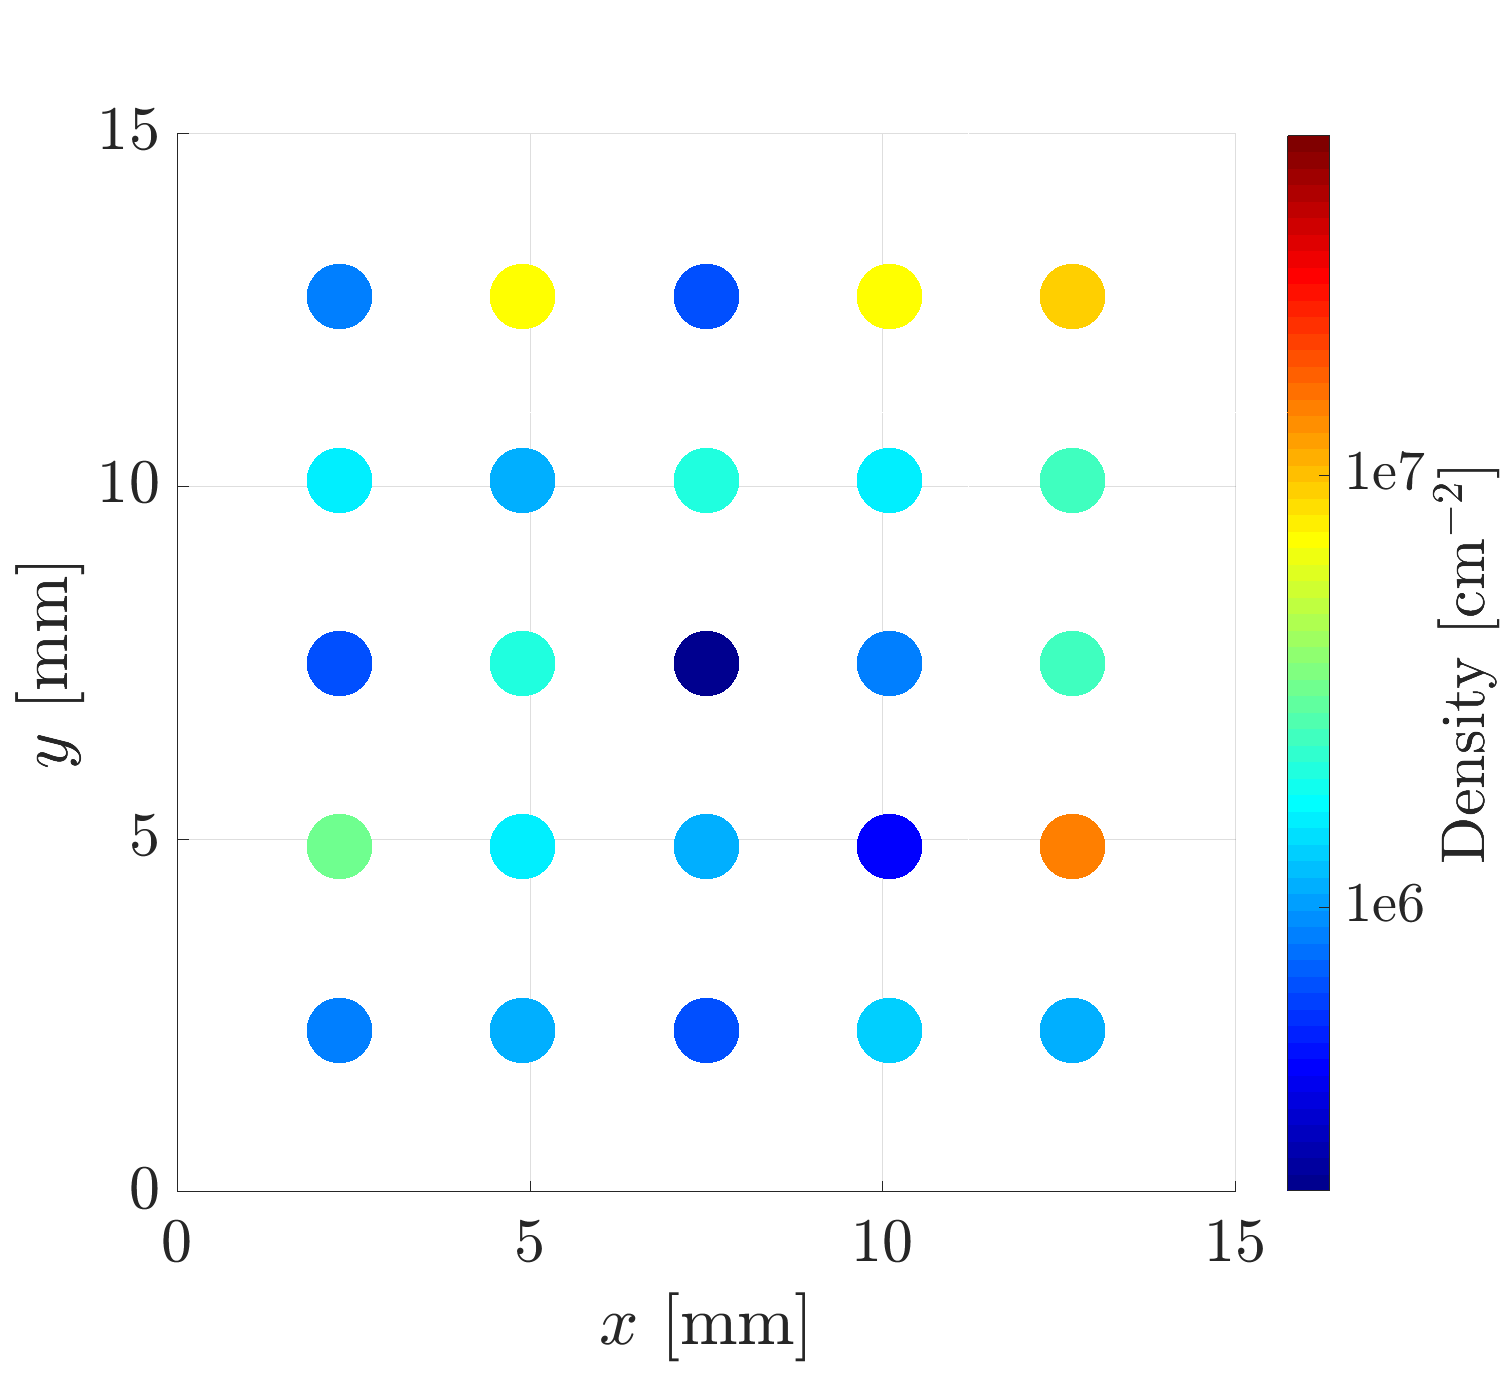
\includegraphics[width=0.8\linewidth]{subCb_densityData.png}
    \caption[Map of the polishing grit density on substrate C after surface pre-growth preparation.]{A map of the polishing grit density at 25 different locations on the $\SI{15}{\milli\metre}\times\SI{15}{\milli\metre}$ substrate C after surface pre-growth preparation. The polishing grit density was observed to vary between \todo{\SI{5e+06}{\particle\centi\metre^{-2}} and \SI{3e+07}{\particle\centi\metre^{-2}}}.}
    \label{fig:subCb_densityData}
\end{figure}


%%=========================================
%\section{AFM Study of Etched Substrate C}
\subsection{Surface Roughness}

Fig.~\ref{fig:subCb_afm}
\begin{figure}[htbp]
    \centering
    \begin{subfigure}[t]{0.032\linewidth}
    \centering
        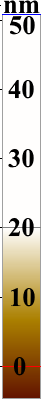
\includegraphics[width=\linewidth]{subCb_afm_scale.png}
        \captionsetup{list=no}
    \end{subfigure}
    \hfill
    \begin{subfigure}[t]{0.3\linewidth}
    \centering
        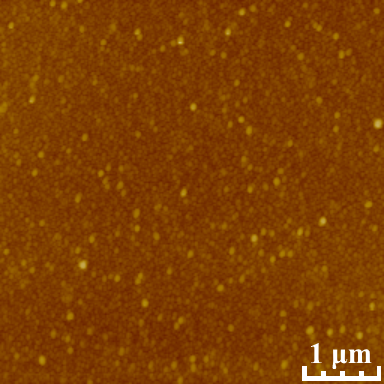
\includegraphics[width=\linewidth]{subCb_afm_centre.png}
        \caption{}\label{fig:subCb_afm_centre}  %\SI{0.85}{\nano\metre}}
    \end{subfigure}%
    \hfill
    \begin{subfigure}[t]{0.3\linewidth}
    \centering
        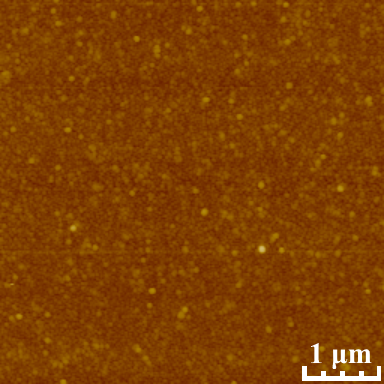
\includegraphics[width=\linewidth]{subCb_afm_upperedge.png}
        \caption{}\label{fig:subCb_afm_edge}  %\SI{0.77}{\nano\metre}}
    \end{subfigure}%
    \hfill
    \begin{subfigure}[t]{0.3\linewidth}
    \centering
        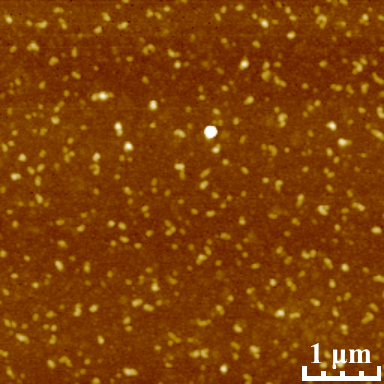
\includegraphics[width=\linewidth]{subCb_afm_upperleftcorner.png}
        \caption{}\label{fig:subCb_afm_corner}  %\SI{1,04}{\nano\metre}}
    \end{subfigure}%
    \caption[\Ac{afm} of substrate C with surface pre-growth preparation.]{\Acf{afm} measurements of substrate C with surface pre-growth preparation. Images of $\SI{5}{\micro\metre}\times\SI{5}{\micro\metre}$ areas are taken at three different locations on the substrate surface: \subref{fig:subCb_afm_centre} near the centre, \ac{rms} roughness \SI{1.4}{\nano\metre}; \subref{fig:subCb_afm_edge} near the upper edge, \ac{rms} roughness \SI{1.4}{\nano\metre}; and \subref{fig:subCb_afm_corner} near the upper left corner, \ac{rms} roughness \SI{2.8}{\nano\metre}.}
    \label{fig:subCb_afm}
\end{figure} % AFM, substrate C, with surface pre-growth preparation.

%%=========================================
\subsection{Impurity Analysis}
\begin{table}[htbp]
    \centering
    \caption[\Ac{eds} impurity analysis of substrate C with surface pre-growth preparation.]{Results of the \acf{eds} impurity analysis at three different locations on the $15\times15$ \SI{}{\milli\metre^2} (211)B \ac{czt} substrate C with surface pre-growth preparation (atomic concentration \%). The X-ray signal is acquired from $\SI{1270}{\micro\metre}\times\SI{890}{\micro\metre}$ areas near the centre, upper edge, and upper left corner.}\label{tab:subCb_eds_analysis}
    \begin{tabu} to 1.0\textwidth { X[1.85,r] X[1.125,c] X[1.125,c] X[1.125,c] X[1.125,c] X[1.125,c] X[1.125,c] X[1.125,c] }
    \hline
         & \textbf{\ce{Te}} (at.\%) & \textbf{\ce{Cd}} (at.\%) & \textbf{\ce{Zn}} (at.\%) & \textbf{\ce{Al} } (at.\%) & \textbf{\ce{Si}} (at.\%) & \textbf{\ce{C}} (at.\%) & \textbf{\ce{O}} (at.\%) \\
        \hline
         Near corner & \SI{45.16}{} & \SI{45.26}{} & \SI{1.40}{} & \SI{1.79}{} & \SI{0.54}{} & \SI{5.85}{} & \SI{0}{} \\ %\SI{1.0}{} & \SI{14.0}{}
         Near edge & \SI{44.91}{} & \SI{44.93}{} & \SI{1.43}{} & \SI{2.33}{} & \SI{0.53}{} & \SI{5.86}{} & \SI{0}{} \\ % \SI{7.5}{} & \SI{14.0}{}
         Near centre & \SI{45.02}{} & \SI{44.88}{} & \SI{1.45}{} & \SI{2.14}{} & \SI{0.52}{} & \SI{6.00}{} & \SI{0}{} \\ % \SI{7.5}{} & \SI{7.5}{} 
         \hline
    \end{tabu}
\end{table}

%%=========================================